\chapter{Đọc thêm 2: Nhập môn Veridical Data Science}
\label{ch:M1L1-reading2}

\section{Nhập môn Khoa học Dữ liệu Chân thực (Veridical Data Science)}

Thực hành khoa học dữ liệu chân thực (veridical data science) chính là thực hành khoa học dữ liệu “đúng đắn” (truthful). Mục tiêu của khoa học dữ liệu chân thực là trả lời các câu hỏi trong thế giới thực bằng cách thu thập và đánh giá một cách phản biện các bằng chứng thực nghiệm (dựa trên dữ liệu) bằng cách sử dụng các đánh giá chủ quan của con người trong bối cảnh kiến thức chuyên ngành. Nếu bằng chứng thực nghiệm được coi là đủ độ tin cậy, nó sẽ được truyền đạt tới các bên liên quan trong lĩnh vực đó, nơi nó có thể đóng vai trò trong việc ra quyết định thực tế và cập nhật kiến thức chuyên ngành.

\begin{tcolorbox}[title={Hộp 1.1: Veridical Data Science}]
Khoa học dữ liệu chân thực (Veridical data science) là hoạt động thực hành phân tích dữ liệu đồng thời đưa ra các đánh giá của con người và sử dụng kiến thức chuyên ngành để trích xuất và truyền đạt thông tin hữu ích và đáng tin cậy từ dữ liệu, nhằm giải quyết một vấn đề thực tiễn trong một lĩnh vực cụ thể.
\end{tcolorbox}

Mục tiêu tổng thể của hầu hết các dự án khoa học dữ liệu là sử dụng những hiểu biết thu được từ các phân tích dữ liệu để giúp chúng ta đưa ra quyết định trong thế giới thực. Ví dụ, các nhà nhân khẩu học tiến hành và phân tích các cuộc khảo sát trên những thành viên của một quần thể người đang được quan tâm để giúp định hướng các quyết định chính sách, các nhà sinh thái học quan sát và phân tích dữ liệu về sự phân bố và hành vi của động vật, thực vật để giúp đưa ra các quyết định bảo tồn, và các nhà phân tích tài chính đánh giá xu hướng thị trường tài chính để giúp đưa ra các quyết định tài chính.

\subsection{Vai trò của Dữ liệu và Thuật toán trong Việc Ra quyết định Thực tiễn}

Việc thu được những hiểu biết sâu sắc từ dữ liệu thường liên quan đến việc triển khai các thuật toán được thiết kế để tóm tắt và trích xuất các mô hình và mối quan hệ có liên quan được ẩn giấu trong một tập dữ liệu. Thuật toán là một tập hợp các lệnh cho máy tính biết cách thực hiện một tác vụ cụ thể (chẳng hạn như tóm tắt một mô hình cụ thể). Vì con người đã chọn tập hợp các lệnh định nghĩa mỗi thuật toán, mỗi thuật toán là một cấu trúc tinh thần (mental construct) nhằm đại diện cho các loại mối quan hệ nhất định mà chúng ta giả thuyết là có ý nghĩa trong dữ liệu của mình. Chúng ta sử dụng thuật ngữ “thuật toán” khá rộng. Ví dụ, ngoài "các thuật toán học máy (ML)", vốn tạo ra các dự đoán về một biến phản hồi, bạn có thể coi việc tính toán giá trị trung bình bằng máy tính như một thuật toán cộng một tập hợp các số lại và sau đó chia cho số lượng các số trong tập hợp đó. Bạn thậm chí có thể coi quá trình tạo biểu đồ phân tán (scatterplot) như một thuật toán trực quan hóa dữ liệu, lấy một tập hợp các cặp số và sắp xếp chúng thành các điểm trong không gian hai chiều.

Sự liên quan của một thuật toán đối với thế giới thực bị giới hạn bởi mức độ mà dữ liệu làm cơ sở cho nó phản ánh thực tế. Đáng tiếc là, dữ liệu hầu như không bao giờ nắm bắt hoàn hảo thế giới thực mà nó được thiết kế để đo lường. Một quy trình thu thập dữ liệu không được cân nhắc kỹ lưỡng hoặc tuân thủ kém có thể dẫn đến một tập dữ liệu không đại diện đầy đủ cho quần thể thực tế dự kiến, và các công cụ đo lường không chính xác cùng các phép tính xấp xỉ của con người có thể dẫn đến các giá trị sai được nhập vào tập dữ liệu. Trừ khi chúng ta biết chắc chắn các giá trị "thực" của từng đại lượng thực tế đang được đo lường là gì (điều mà chúng ta thường không biết, vì chúng ta chỉ nhìn thấy các phép đo lường của chính mình về các đại lượng này), chúng ta thường không biết các giá trị trong bất kỳ tập dữ liệu nhất định nào chính xác đến mức nào. Hơn nữa, ngay cả khi dữ liệu ban đầu của chúng ta là một sự phản ánh hợp lý của thực tế, khi chúng ta làm sạch và tiền xử lý dữ liệu để có thể thực hiện các tính toán, chúng ta đã sửa đổi nó. Mặc dù các sửa đổi này thường nhằm mục đích đưa dữ liệu của chúng ta đến gần hơn với thực tế, nhưng chúng lại dựa trên các phán đoán và giả định của chính chúng ta về các đại lượng thực tế mà các phép đo trong dữ liệu của chúng ta được cho là đại diện. Tuy nhiên, các giả định sai lầm có thể vô tình làm giảm đi mối liên hệ giữa dữ liệu của chúng ta và thực tế.

Tuy nhiên, những vấn đề này không chỉ liên quan đến dữ liệu hiện tại mà chúng ta sử dụng để tiến hành phân tích và huấn luyện các thuật toán, chúng cũng đúng với dữ liệu trong tương lai mà chúng ta sẽ áp dụng các thuật toán đó. Ví dụ, mặc dù một nhà nhân khẩu học có thể đã phân tích một cuộc khảo sát liên quan đến 500 người Mỹ, nhưng mục tiêu cuối cùng là sử dụng thông tin này để giúp hiểu và đưa ra các quyết định trong tương lai cho tất cả người Mỹ (trong trường hợp này, dữ liệu hiện tại tương ứng với 500 người Mỹ tham gia khảo sát vào ngày khảo sát được thực hiện, và dữ liệu trong tương lai tương ứng với tất cả người Mỹ trong một khoảng thời gian sau cuộc khảo sát). Tương tự, một nhà phân tích tài chính có thể huấn luyện một thuật toán để dự đoán xu hướng thị trường tài chính dựa trên dữ liệu từ 10 năm qua, nhưng mục tiêu của họ là áp dụng thuật toán đó để dự đoán và hiểu các xu hướng thị trường trong tương lai. Trong mỗi trường hợp, dữ liệu tương lai được sử dụng để đưa ra các quyết định trong thế giới thực tương tự như — nhưng chắc chắn không giống hệt với — dữ liệu hiện tại được sử dụng để tiến hành phân tích và khớp các thuật toán.

Do đó, nếu chúng ta muốn các quyết định thực tế mà chúng ta đưa ra dựa trên các thuật toán là đáng tin cậy, chúng ta cần dữ liệu hiện tại làm nền tảng cho các thuật toán của chúng ta và dữ liệu tương lai mà chúng ta muốn áp dụng chúng phản ánh thực tế một cách hợp lý và tương tự nhau.\footnote{Có toàn bộ một lĩnh vực Học máy (ML) gọi là học chuyển giao (transfer learning) liên quan đến việc áp dụng các thuật toán vào các vấn đề liên quan tương tự (nhưng không giống hệt) với vấn đề hiện tại. Điều này cũng bao gồm việc thích ứng miền (domain adaptation) liên quan đến dữ liệu tương lai không giống với dữ liệu hiện tại.} Chúng ta cũng cần các thuật toán mà chúng ta huấn luyện có thể nắm bắt một cách đáng tin cậy các mô hình và mối quan hệ có chứa trong cả dữ liệu hiện tại và tương lai. Tức là, chúng ta cần những kết nối mạnh mẽ giữa ba cảnh giới (Hình \ref{fig:three_realms}), đó là (1) cảnh giới thế giới thực (nơi chúng ta sinh sống); (2) cảnh giới dữ liệu (vốn là một sự xấp xỉ của thực tế và là nơi dữ liệu của chúng ta tồn tại); và (3) cảnh giới thuật toán (nơi tồn tại các thuật toán là các cấu trúc tinh thần được thiết kế để đại diện cho dữ liệu của chúng ta).

\begin{figure}[htbp]
    \centering
    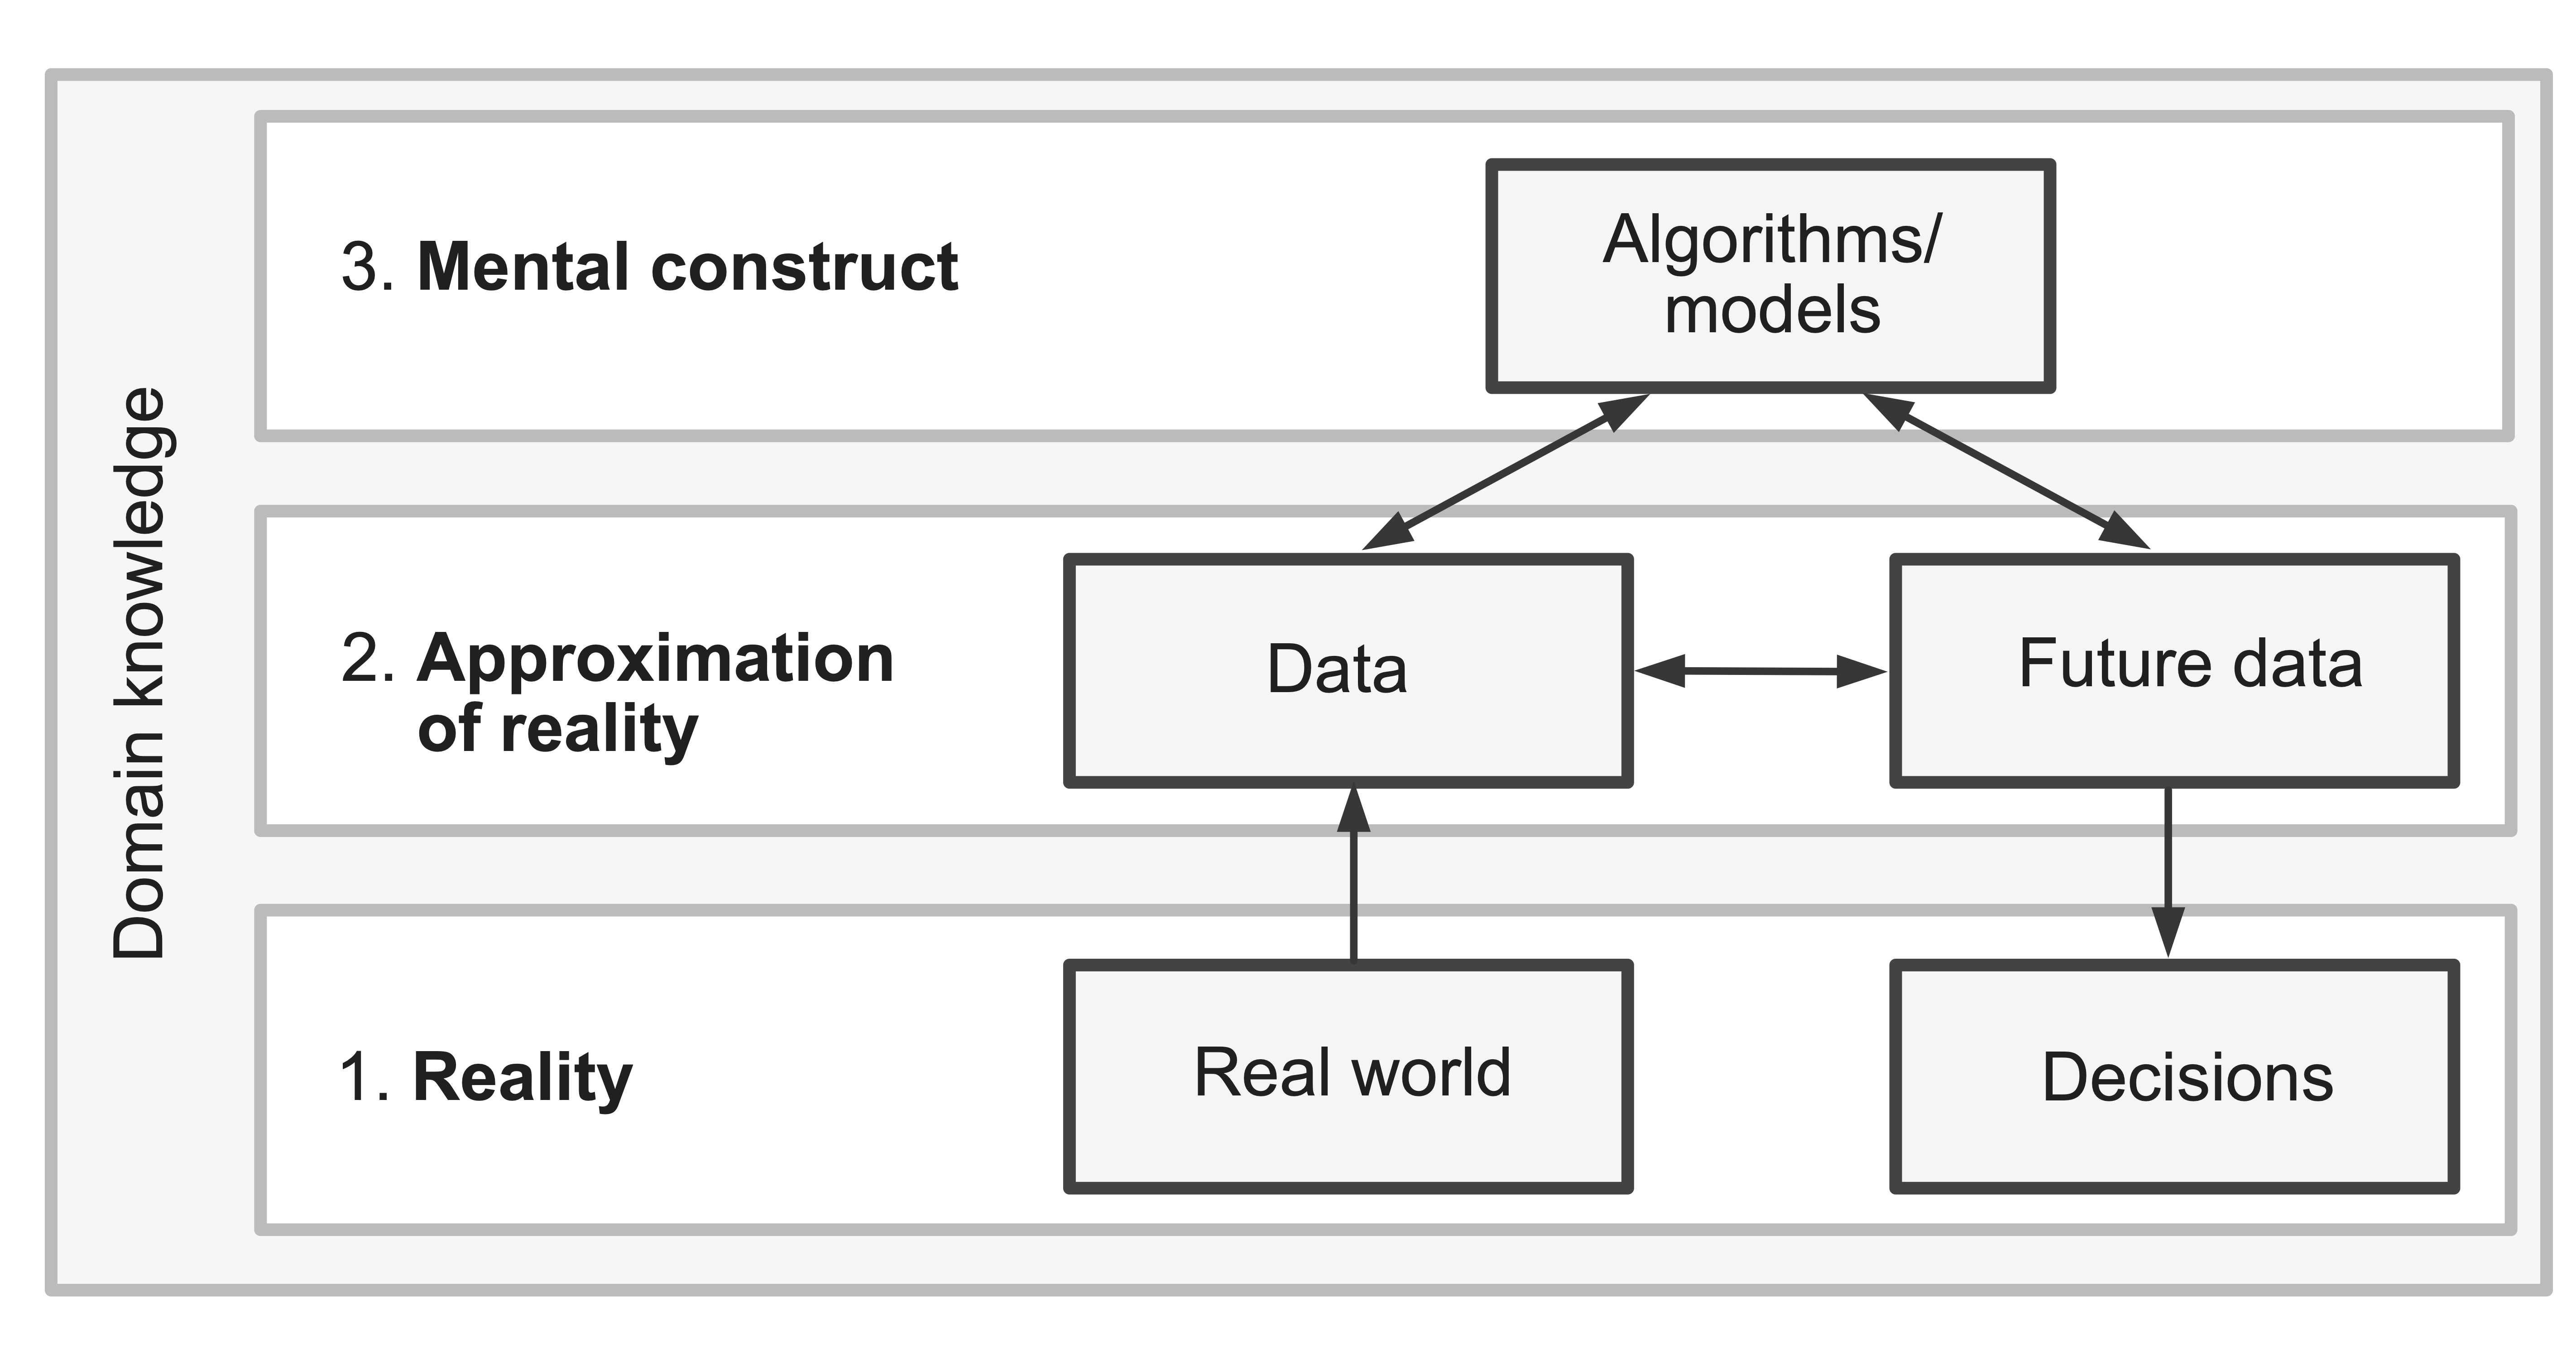
\includegraphics[width=0.8\textwidth]{gfx/m1l1_vds_fig1-1_three_realms.png}
    \caption{Ba cảnh giới: thực tế, một sự xấp xỉ của thực tế (nơi dữ liệu của chúng ta tồn tại), và cảnh giới cấu trúc tinh thần (nơi các phân tích và thuật toán của chúng ta tồn tại).}
    \label{fig:three_realms}
\end{figure}

Vấn đề là chúng ta thường không biết các kết nối giữa ba cảnh giới này mạnh đến mức nào, và việc đưa ra các quyết định thực tế dựa trên kết quả từ các thuật toán không đại diện cho thực tế (cho dù là do dữ liệu là một xấp xỉ kém của thực tế hay do sử dụng các kỹ thuật phân tích không đúng cách) có thể dẫn đến những kết quả không đáng tin cậy với hậu quả thực tiễn nghiêm trọng. Hãy xem xét ví dụ về phần mềm nhận dạng khuôn mặt. Đã có nhiều tài liệu ghi nhận rằng nhiều ứng dụng phần mềm được thiết kế để nhận dạng khuôn mặt bằng hình ảnh hoạt động tốt hơn nhiều khi nhận diện khuôn mặt của người da sáng so với người da sẫm. Một trong những nguyên nhân chính của vấn đề này là các thuật toán này được xây dựng chủ yếu bằng hình ảnh của những người có làn da sáng (tức là, dữ liệu không phản ánh sự đa dạng tồn tại trong thế giới thực) (Khalil et al. 2020). Khi dữ liệu bị thiên lệch được sử dụng để đào tạo phần mềm nhận dạng khuôn mặt, phần mềm thu được thường cũng sẽ bị thiên lệch, và khi được sử dụng trong thế giới thực, những thiên lệch này có thể dẫn đến việc làm trầm trọng thêm các bất bình đẳng xã hội hiện có.

Vì dữ liệu của bạn sẽ không thông báo cho bạn biết liệu nó có đại diện chính xác cho thực tế hay không, và các thuật toán của bạn cũng sẽ không cảnh báo bạn khi chúng được sử dụng không đúng cách, bạn cần phải thực hiện công việc của một "thám tử dữ liệu" (tư duy phản biện) để xác định xem dữ liệu của bạn có phải là một phản ánh hợp lý của thực tế hay không và liệu các thuật toán của bạn có đang được áp dụng phù hợp với dữ liệu và vấn đề chuyên ngành của bạn hay không. Trong các phần tiếp theo, chúng tôi sẽ giới thiệu một số câu hỏi tư duy phản biện giúp bạn sử dụng kiến thức chuyên ngành liên quan để đánh giá độ tin cậy của các kết quả dựa trên dữ liệu một cách định tính, thông qua việc xem xét mức độ dữ liệu phản ánh thực tế chính xác đến đâu và mức độ phân tích và thuật toán phù hợp với ngữ cảnh của dữ liệu và vấn đề. Sau đó, chúng tôi sẽ giới thiệu các nguyên tắc về khả năng dự đoán (predictability), khả năng tính toán (computability) và tính ổn định (stability) – gọi chung là PCS, mà chúng tôi sẽ sử dụng xuyên suốt cuốn sách này để đánh giá độ tin cậy của các kết quả dựa trên dữ liệu một cách định lượng, xét về khía cạnh mức độ áp dụng của kết quả đối với các kịch bản dữ liệu tương lai có liên quan và mức độ nhạy cảm của chúng đối với các nhiễu động hợp lý trong dữ liệu và quy trình phân tích của chúng ta (bao gồm cả các phán đoán của con người mà chúng ta đưa ra khi làm sạch, tiền xử lý và phân tích dữ liệu).

\subsection{Đánh giá và Xây dựng Độ tin cậy Bằng Tư duy Phản biện}

Khoa học dữ liệu không chỉ bao gồm việc làm toán và viết mã; nó còn đòi hỏi kỹ năng tư duy phản biện mạnh mẽ và nền tảng kiến thức chuyên ngành liên quan đến dự án mà bạn đang thực hiện (có thể thu được từ chuyên môn của chính bạn, internet, sách hoặc từ các cộng tác viên). Những kỹ năng này rất quan trọng để xác định các điểm yếu tiềm ẩn trong các kết nối giữa ba cảnh giới, được mô tả ở trên, và để phát hiện những thiên lệch có thể len lỏi vào quy trình thu thập và phân tích dữ liệu. Nếu không có kỹ năng tư duy phản biện vững vàng và kiến thức chuyên ngành cơ bản (thậm chí nếu chỉ là từ việc đánh giá tài liệu), bạn có nguy cơ tạo ra những kết quả gây hiểu lầm, có thể mang lại hậu quả thực tế thảm khốc.

Thật không may, số liệu thống kê và phân tích dữ liệu có tiếng xấu về độ tin cậy trong công chúng, với những câu nói như "Có ba loại nói dối: nói dối, nói dối tồi tệ và thống kê"\footnote{Việc sử dụng từ "thống kê" ở đây theo nghĩa thông tục thực chất có nghĩa là "phân tích dữ liệu".} thường làm gián đoạn các cuộc thảo luận thông thường về phân tích dữ liệu. Dù chúng tôi rất muốn nói rằng danh tiếng này là không đáng có, chúng ta không thể phủ nhận rằng rất dễ sử dụng dữ liệu để nói dối. Vấn đề là hầu hết thời gian, những lời nói dối này là vô ý, xuất phát từ việc thiếu tư duy phản biện và không xem xét kỹ lưỡng các kết quả có được từ dữ liệu (ví dụ: bằng cách sử dụng các nguyên tắc PCS mà chúng tôi sẽ giới thiệu dưới đây) trước khi trình bày chúng như là những "sự thật".

Một nhà khoa học dữ liệu thành thạo về tư duy phản biện và kiến thức chuyên ngành (và/hoặc làm việc chặt chẽ với các chuyên gia), người có hiểu biết hợp lý về các thuật toán đang được sử dụng (bao gồm các giả định và cạm bẫy liên quan), và nắm vững các nguyên tắc của PCS, sẽ ít có khả năng rơi vào cái bẫy vô tình nói dối bằng dữ liệu. Lần tới khi bạn nghe ai đó nói, “Có ba loại nói dối: nói dối, nói dối tồi tệ và thống kê,” thay vì cảm thấy bị xúc phạm, bạn có thể sửa lại: “Có ba loại nói dối: nói dối, nói dối tồi tệ và thống kê tồi.” Không phải tất cả các dự án khoa học dữ liệu đều liên quan đến phân tích dữ liệu tồi, nhưng chắc chắn là có một số!

Một số kỹ thuật tư duy phản biện mà chúng tôi khuyến nghị áp dụng trong suốt mọi dự án khoa học dữ liệu (và để đánh giá dự án của người khác) bao gồm:

\begin{itemize}
    \item \textbf{Đặt câu hỏi về vấn đề thực tiễn.} Câu hỏi đang được đặt ra có thực sự là câu hỏi mà bạn quan tâm không, và câu hỏi này ngay từ đầu có đạo đức không? Ví dụ, nếu bạn nhận được câu hỏi kinh doanh "Chúng ta có thể thay đổi tính năng nào trên trang web để khiến khách hàng ít hủy đăng ký hơn?", bạn có thể thấy rằng một câu trả lời là chuyển nút "Hủy đăng ký" đến một vị trí kín đáo hơn (tức là khó tìm hơn). Nhưng đây có thực sự là câu hỏi mà bạn muốn hỏi không? Nó có đạo đức không? Một câu hỏi tốt hơn có thể là, “Tại sao khách hàng lại có xu hướng hủy đăng ký sản phẩm của chúng ta?” Câu trả lời cho câu hỏi đó có thể giúp công ty của bạn cải thiện các dịch vụ sản phẩm (thay vì chỉ gây khó khăn cho khách hàng trong việc hủy).
    \item \textbf{Đặt câu hỏi về dữ liệu.} Dữ liệu đến từ đâu? Nguồn dữ liệu có đáng tin cậy không? Dữ liệu có liên quan đến câu hỏi đang được đặt ra, cũng như bất kỳ bối cảnh tương lai nào mà kết quả có thể được áp dụng không? Các giá trị chứa trong dữ liệu thực sự tương ứng với điều gì trong thế giới thực? Những câu hỏi này là một cách tuyệt vời để nắm bắt những điểm không nhất quán và lỗi có thể làm chệch hướng phân tích của bạn. Hãy thử tưởng tượng bản thân bạn có mặt trực tiếp trong quá trình thu thập dữ liệu. Các vấn đề tiềm ẩn nào có thể phát sinh? Bất cứ khi nào có thể, hãy làm công việc "mòn giày" (shoe-leather work) (Freedman 1991).
    \item \textbf{Đặt câu hỏi về phân tích, thuật toán và kết quả.} Những kết quả này có ý nghĩa gì trong bối cảnh thực tế? Chúng có hợp lý không? Phân tích và thuật toán có đưa ra bất kỳ giả định nào về dữ liệu hay lĩnh vực không? Những giả định này có hợp lý không? Những kết quả này có trả lời được câu hỏi chính của dự án không? Các kết quả có được truyền đạt một cách chính xác không?
\end{itemize}

Ngoài những câu hỏi này, điều quan trọng là phải theo dõi thiên kiến xác nhận (confirmation bias) và thiên kiến mong muốn (desirability bias). Thiên kiến xác nhận xảy ra khi bạn không xem xét kỹ lưỡng các kết quả một cách phản biện vì chúng khớp với những gì bạn mong đợi tìm thấy. Là con người, chúng ta có nhiều khả năng sẽ kiểm tra kỹ và soi xét kết quả khi chúng không khớp với kỳ vọng của mình (điều đó có nghĩa là chúng ta ít có khả năng phát hiện lỗi khi kết quả khớp với những gì chúng ta mong đợi). Thiên kiến mong muốn xảy ra khi bạn cố gắng tìm ra kết quả mà bạn nghĩ người khác (hoặc dư luận) mong đợi bạn tìm thấy.

Bạn có thể làm gì để giảm thiểu rủi ro của thiên kiến xác nhận và mong muốn? Mặc dù không thể hoàn toàn gạt bỏ kỳ vọng của bạn, bạn có thể rèn luyện một sự hoài nghi lành mạnh đối với mọi kết quả bạn nhận được, bất kể nó có khớp với những gì bạn hoặc người khác mong đợi hay muốn tìm thấy hay không.

\subsubsection{Nghiên cứu điển hình: Ước tính số động vật chết do cháy rừng ở Úc năm 2019}
Chúng ta hãy sử dụng các kỹ năng tư duy phản biện của mình để làm công việc thám tử, sử dụng một ví dụ từ thảm họa cháy rừng tàn phá hơn 42 triệu mẫu Anh ở bờ biển phía đông nước Úc trong nhiều tháng vào cuối năm 2019 và sang năm 2020 (để dễ hình dung, diện tích này lớn hơn toàn bộ tiểu bang Florida). Một số nhà khoa học (nổi bật nhất là Giáo sư Chris Dickman tại Đại học Sydney, người có hơn 30 năm kinh nghiệm nghiên cứu về sinh thái học, bảo tồn và quản lý động vật có vú ở Úc) ước tính rằng "hơn 1 tỷ động vật đã chết trong các vụ hỏa hoạn." Con số 1 tỷ đó là vô cùng kinh ngạc. Mặc dù hầu hết mọi người sẽ chấp nhận các báo cáo của các nghiên cứu khoa học mà không thắc mắc, chúng ta không phải là hầu hết mọi người. Hãy dành thời gian suy nghĩ nghiêm túc về nguồn gốc của con số gây kinh ngạc này, 1 tỷ, có thể đến từ đâu (không phải để hạ thấp những hậu quả kinh hoàng không thể phủ nhận của các vụ hỏa hoạn này, mà đúng hơn là để hiểu chúng rõ hơn).

\paragraph{Đặt câu hỏi về dữ liệu}

Bạn nghĩ dữ liệu làm cơ sở cho tuyên bố rằng "1 tỷ động vật đã chết trong các vụ hỏa hoạn" được thu thập như thế nào? Có phải có một nhóm các nhà khoa học đang đếm thủ công từng con vật đã chết không? Thuật ngữ "động vật" có bao gồm côn trùng, chẳng hạn như kiến và ruồi không? May mắn thay, với một chút nghiên cứu, chúng tôi đã có thể tìm thấy câu trả lời cho những câu hỏi này khá nhanh chóng. Chúng tôi khuyến khích bạn thử trả lời bất kỳ câu hỏi nào của riêng bạn. Một cuộc tìm kiếm nhanh trên internet dẫn chúng tôi đến một bài báo (Đại học Sydney 2020), trong đó tuyên bố rằng Giáo sư Dickman đã dựa trên các ước tính của mình từ một nghiên cứu chi tiết của Johnson và cộng sự (2007) (13 năm trước khi vụ hỏa hoạn xảy ra) mà Giáo sư Dickman là đồng tác giả:

"Các số liệu được Giáo sư Dickman trích dẫn dựa trên báo cáo năm 2007 của Quỹ Quốc tế Bảo vệ Thiên nhiên (WWF) về tác động của việc phát quang đất đối với động vật hoang dã ở New South Wales... [trong đó có] các ước tính về mật độ quần thể động vật có vú, chim và bò sát ở NSW" (Đại học Sydney 2020).

Bản sao PDF của cả hai bài báo này (Johnson et al. 2007) và (Đại học Sydney 2020) được cung cấp trong thư mục bushfires/ của kho lưu trữ GitHub bổ sung cho bạn đọc quan tâm.

Những gì chúng tôi tìm thấy trong quá trình tìm kiếm tài liệu của mình là những ước tính này dựa trên dữ liệu được thu thập vào năm 2007, và khi đọc thêm, chúng tôi phát hiện ra rằng nghiên cứu này chỉ bao phủ một khu vực nhỏ của bang New South Wales. Báo cáo từ Đại học Sydney (2020) cũng tuyên bố rằng "con số này bao gồm động vật có vú (không bao gồm dơi), chim và bò sát và không bao gồm ếch, côn trùng hoặc các động vật không xương sống khác."

Từ thông tin này, chúng ta có thể kết luận rằng những kết quả này không dựa trên một cơ sở dữ liệu thần bí nào đó chứa thông tin về tất cả các động vật đã chết trong hỏa hoạn, rất có thể vì không có dữ liệu nào như vậy tồn tại (và việc cố gắng tưởng tượng việc thu thập một tập dữ liệu như vậy sẽ nhanh chóng dẫn chúng ta đến kết luận rằng đây sẽ là một nhiệm vụ bất khả thi). Mặc dù dữ liệu làm nền tảng cho các kết quả đến từ một nguồn có thể xác minh và hợp pháp (nghiên cứu năm 2007 do Tổ chức Động vật Hoang dã Thế giới, một tổ chức uy tín thực hiện), điều này không tự động có nghĩa là nó liên quan đến câu hỏi đang được đặt ra. Rất nhiều thứ có thể thay đổi trong 13 năm, và thật là một tuyên bố lớn khi nói rằng các ước tính được thu thập từ một môi trường sống nhỏ, cục bộ có thể được khái quát hóa cho toàn bộ khu vực bị ảnh hưởng bởi hỏa hoạn.

Do đó, dữ liệu làm nền tảng cho nghiên cứu này là có liên quan, nhưng không nghi ngờ gì về việc nó bị hạn chế về phạm vi. Cuối cùng, Giáo sư Dickman đã làm hết sức mình với một tập dữ liệu hiện có mà ông đã quen thuộc, vì không có dữ liệu liên quan nào khác có sẵn. Thông thường, dữ liệu tốt nhất chỉ là dữ liệu bạn đang có.

\paragraph{Đặt câu hỏi về phân tích}

Với việc dữ liệu chỉ dựa trên một khu vực nhỏ, cục bộ, Giáo sư Dickman và các cộng sự của ông đã sử dụng dữ liệu như thế nào để ước tính số lượng động vật đã chết trên toàn bộ khu vực bị ảnh hưởng? Từ báo cáo của Đại học Sydney (2020), chúng ta biết được rằng

"Ước tính về mật độ quần thể động vật có vú, chim và bò sát ở NSW [thu được bằng cách nhân] các ước tính mật độ với diện tích thảm thực vật được phép phát quang" (Đại học Sydney 2020).

Chúng tôi giải thích điều này có nghĩa là họ đã lấy các ước tính năm 2007 về mật độ động vật và phóng to những con số này dựa trên kích thước của khu vực bị ảnh hưởng. Cách tiếp cận này rõ ràng không tính đến sự khác biệt về mật độ động vật trên toàn bộ khu vực bị ảnh hưởng, cũng như không tính đến cách các mật độ này có thể đã thay đổi theo thời gian. Tuy nhiên, vì không có thêm dữ liệu nào, họ có thể làm gì khác?

Mặc dù chúng ta có thể chỉ trích các kết luận dựa trên dữ liệu của người khác bao nhiêu tùy thích, nhưng trong nhiều trường hợp, đó là những con số tốt nhất (và thường là duy nhất) hiện có. Khi chỉ trích nghiên cứu của người khác, hãy luôn ghi nhớ rằng đằng sau mọi kết luận dựa trên dữ liệu là một con người có ý định tốt với những cảm xúc (điều mà mọi người thường cố tình quên). Trong trường hợp nghiên cứu của Giáo sư Dickman, mặc dù có lẽ chúng ta không nên lấy các tuyên bố như một sự thật cơ bản (chính các tác giả đã rất rõ ràng trong báo cáo của họ rằng đây là những ước tính thô và không nên hiểu theo nghĩa đen), chúng thực sự vẽ nên một bức tranh tác động sâu sắc về hậu quả tàn khốc của các vụ hỏa hoạn đối với các quần thể động vật địa phương dựa trên thông tin có sẵn. Hơn nữa, đây là nghiên cứu tầm cỡ đầu tiên thậm chí đã cố gắng định lượng tác động của các vụ hỏa hoạn đối với quần thể động vật.\footnote{Vào cuối năm 2020, một nghiên cứu mới của WWF (do Giáo sư Chris Dickman giám sát và Tiến sĩ Lily Van Eeden dẫn đầu) đã cập nhật con số này để báo cáo rằng số lượng động vật chết trong các vụ hỏa hoạn có khả năng gần 3 tỷ, một con số thậm chí còn tàn khốc hơn so với báo cáo trước đó (Vernick 2020). Nghiên cứu này chia nhỏ con số đó thành "143 triệu động vật có vú, 2,46 tỷ loài bò sát, 180 triệu loài chim và 51 triệu con ếch." Báo cáo cập nhật này chứng minh rằng các số liệu được báo cáo ban đầu không nên được hiểu theo nghĩa đen, mà thay vào đó, chúng đóng vai trò vẽ ra bức tranh tổng quát về mức độ nghiêm trọng của sự tàn phá đối với động vật hoang dã ở miền đông nước Úc.}

Bằng cách suy nghĩ phản biện về các con số được báo cáo liên quan đến tác động của các vụ hỏa hoạn này, chúng ta có thể hiểu rõ hơn nhiều về nguồn gốc của chúng và cách chúng ta nên diễn giải chúng. Trong các nghiên cứu của riêng bạn, lời khuyên của chúng tôi là hãy luôn minh bạch về các giả định làm nền tảng cho dữ liệu và kết quả của bạn và ghi chép lại chúng (công khai, nếu có thể). Mọi kết quả dựa trên dữ liệu đều có những cảnh báo (caveats), và công việc của bạn là đảm bảo rằng kết quả của mình đang được diễn giải chính xác nhất có thể.

\subsection{Đánh giá và Xây dựng Độ tin cậy Bằng Khung PCS}

Mặc dù những câu hỏi tư duy phản biện này giúp cung cấp một thước đo định tính chung về độ tin cậy của các kết quả dựa trên dữ liệu, việc cung cấp các thước đo định lượng thường cũng rất quan trọng. Đây là lúc các nguyên tắc về khả năng dự đoán (predictability), khả năng tính toán (computability) và tính ổn định (stability) – gọi chung là PCS, phát huy tác dụng. Những nguyên tắc này lần đầu tiên được giới thiệu trong Yu và Kumbier (2020), nhưng đã được mở rộng rất nhiều trong cuốn sách này.

Khung PCS cung cấp hướng dẫn và kỹ thuật để chứng minh theo kinh nghiệm rằng kết quả của bạn vượt qua một số bài kiểm tra thực tế về dự đoán và đánh giá độ ổn định nhằm giải quyết nhiều nguồn không chắc chắn liên quan đến kết quả của bạn. Ba nguyên tắc PCS là:

\begin{itemize}
    \item \textbf{Khả năng dự đoán (Predictability).} Các kết luận của bạn được coi là có thể dự đoán được nếu bạn có thể chỉ ra rằng chúng xuất hiện lại trong dữ liệu tương lai có liên quan và/hoặc phù hợp với kiến thức chuyên ngành hiện có. Các đánh giá khả năng dự đoán có thể được coi như một bài kiểm tra thực tế (reality check). Chúng tôi sẽ mở rộng nguyên tắc dự đoán trong phần tiếp theo.
    \item \textbf{Khả năng tính toán (Computability).} Khả năng tính toán là nền tảng cốt lõi cho mọi phân tích dữ liệu, đánh giá PCS và các nghiên cứu mô phỏng. Thông thường, bạn không cần phải chứng minh rằng kết quả của mình có thể tính toán được; đúng hơn là bạn sẽ sử dụng máy tính để tiến hành và đánh giá các phân tích của mình, cũng như để tạo ra các mô phỏng lấy cảm hứng từ dữ liệu.
    \item \textbf{Tính ổn định (Stability).} Kết quả của bạn được coi là ổn định nếu bạn có thể chỉ ra rằng chúng vẫn khá nhất quán khi có những sửa đổi (nhiễu động - perturbations) thực tế được thực hiện đối với dữ liệu cơ sở, các quyết định đánh giá và các lựa chọn thuật toán. Đánh giá tính ổn định có thể được coi là một tập hợp các bài kiểm tra áp lực (stress-test) đối với tính không chắc chắn liên quan đến kết quả dựa trên dữ liệu của bạn.\footnote{Lưu ý rằng khả năng dự đoán có thể được coi là một trường hợp đặc biệt của tính ổn định khi nhiễu động của dữ liệu hiện tại chính là dữ liệu tương lai.}
\end{itemize}

\begin{tcolorbox}[title={Hộp 1.2: Khung PCS}]
Khung PCS (khả năng dự đoán, khả năng tính toán và tính ổn định) cung cấp các hướng dẫn để đánh giá thực nghiệm độ tin cậy của các bằng chứng thu được từ dữ liệu ở mọi bước trong vòng đời khoa học dữ liệu (DSLC). Áp dụng các nguyên tắc PCS liên quan đến việc sử dụng các khám phá tính toán để đảm bảo kết quả của bạn có thể dự đoán được và ổn định.
\end{tcolorbox}

Các đánh giá khả năng dự đoán và độ ổn định là một phương tiện mạnh mẽ để cung cấp bằng chứng cho độ tin cậy của kết quả dựa trên dữ liệu của bạn. Tuy nhiên, chúng không cho phép bạn chứng minh rằng các kết quả dựa trên dữ liệu của bạn là chắc chắn hoàn toàn. Việc chứng minh tuyệt đối sẽ yêu cầu đánh giá khả năng dự đoán và độ ổn định một cách cạn kiệt, xem xét tất cả các kịch bản phân tích và dữ liệu thay thế có thể có — một nhiệm vụ bất khả thi. Những ý tưởng này chứa đựng tiếng vang của "Sự chứng ngụy Popper" (Popperian falsification), như được định nghĩa bởi nhà triết học Karl Popper vào những năm 1930 (Popper 2002). Chứng ngụy Popper\footnote{Trong triết học của Popper, để một phát hiện được coi là "khoa học", nó phải có "khả năng bị chứng ngụy" (falsifiable); tức là phải có thể bác bỏ nó nếu thực sự nó sai.} nói rằng một phát hiện khoa học không bao giờ thực sự được chứng minh, mà thay vào đó, mỗi kết quả thực nghiệm tích cực đều đưa ra thêm bằng chứng cho phát hiện khoa học đó.

Mặc dù bản thân khung PCS là mới, nhiều ý tưởng làm nền tảng cho nó không mới. Khung PCS nhằm mục đích thống nhất, hợp lý hóa và mở rộng các thực tiễn và ý tưởng tốt nhất từ Học máy (ML), thống kê và khoa học.

\subsubsection{Khả năng dự đoán (Predictability)}
Các nhà khoa học đã tiến hành kiểm tra thực tế khả năng dự đoán trong nhiều thế kỷ. Ví dụ, vào đầu những năm 1800, Carl Friedrich Gauss đã phát triển một mô hình dự đoán vị trí của tiểu hành tinh Ceres trên bầu trời và ông đã kiểm tra mô hình của mình (tức là ông cho thấy nó tạo ra kết quả có thể dự đoán được) bằng cách chứng minh rằng nó dự đoán chính xác vị trí tương lai thực tế của Ceres. Trong môi trường hiện đại hơn, cộng đồng Học máy (ML) từ lâu đã chứng minh khả năng dự đoán bằng cách đánh giá hiệu suất thuật toán của họ trên các tập kiểm chứng và tập kiểm tra (test/validation sets) được giữ lại. Nguyên tắc dự đoán của khung PCS mở rộng vai trò của kiến thức chuyên ngành và việc sử dụng tập kiểm chứng một cách rộng rãi, vượt ra ngoài các bài toán dự báo đơn thuần.

\begin{tcolorbox}[title={Hộp 1.3: Khả năng dự đoán}]
Kết quả dựa trên dữ liệu có thể dự đoán được nếu chúng có thể được chứng minh là xuất hiện lại (tức là có thể được khái quát hóa) trong các kịch bản mới, có liên quan. Bằng chứng mạnh mẽ về khả năng dự đoán có thể thu được bằng cách chứng minh rằng các kết quả vẫn đúng trong bối cảnh dữ liệu thực tế trong tương lai hoặc bên ngoài mà bạn sẽ áp dụng kết quả của mình. Khi không có sẵn dữ liệu tương lai/bên ngoài, một tập kiểm chứng (validation set) thay thế có thể được sử dụng để đánh giá kết quả. Bằng chứng bổ sung về khả năng dự đoán có thể thu được bằng cách chứng minh rằng các phân tích và thuật toán của bạn có khả năng khám phá ra những kết quả và mối quan hệ đã được biết đến rõ ràng trong lĩnh vực chuyên môn.
\end{tcolorbox}

Tuy nhiên, kỹ thuật đánh giá khả năng dự đoán mạnh mẽ nhất liên quan đến việc chứng minh rằng kết quả của bạn xuất hiện lại trong bối cảnh dữ liệu tương lai hoặc bên ngoài thực tế mà bạn sẽ áp dụng chúng. Ví dụ: nếu bạn đã phát triển một thuật toán dự đoán giá cổ phiếu (dựa trên dữ liệu thị trường chứng khoán trong quá khứ) và bạn muốn sử dụng thuật toán của mình để dự đoán giá cổ phiếu tương lai, bạn nên chứng minh rằng thuật toán của bạn tạo ra các dự đoán chính xác cho dữ liệu thị trường chứng khoán trong một khoảng thời gian diễn ra sau thời điểm của dữ liệu ban đầu được sử dụng để "huấn luyện" thuật toán. Lấy một ví dụ khác, hãy tưởng tượng rằng bạn đang tiến hành một phân tích để cố gắng hiểu các yếu tố rủi ro nhiễm trùng tại bệnh viện bằng cách sử dụng dữ liệu thu thập từ các bệnh nhân tại bệnh viện nơi bạn làm việc. Nếu bạn định áp dụng những phát hiện của mình cho bệnh nhân từ các bệnh viện khác, thì bạn nên chứng minh rằng các yếu tố rủi ro mà bạn đã xác định cũng có liên quan đến bệnh nhân ở các bệnh viện khác.

Tuy nhiên, có nhiều tình huống bạn không có quyền truy cập vào bất kỳ dữ liệu bên ngoài hoặc tương lai nào phản ánh bối cảnh mà bạn định áp dụng kết quả hoặc thuật toán của mình. Trong những tình huống này, bạn có thể mô phỏng dữ liệu tương lai hoặc bên ngoài bằng cách giữ lại một phần dữ liệu ban đầu của mình trước khi tiến hành phân tích với mục đích duy nhất là đánh giá khả năng dự đoán cho kết quả của bạn. Dữ liệu bị giữ lại này có thể đóng vai trò như một dữ liệu thay thế (surrogate) cho dữ liệu tương lai. Bằng chứng bổ sung về khả năng dự đoán cho kết quả của bạn có thể thu được từ việc chứng minh rằng các phân tích và thuật toán của bạn có khả năng nắm bắt các kết quả và mối quan hệ được biết đến rõ ràng trong lĩnh vực (xem mục bằng chứng chuyên môn).

\paragraph{Tập dữ liệu Huấn luyện, Kiểm chứng và Kiểm tra}

Trong trường hợp không có sẵn dữ liệu tương lai/bên ngoài, kỹ thuật được khuyên dùng để tạo các tập dữ liệu thay thế cho bên ngoài/tương lai là chia dữ liệu của bạn thành một tập huấn luyện (training set) và một tập kiểm chứng (validation set) (và có thể cả tập kiểm tra - test set), như phổ biến trong cộng đồng ML.

Tập huấn luyện (dữ liệu huấn luyện/tập dữ liệu huấn luyện) là phần lớn nhất của dữ liệu (nên chứa ít nhất 50\% dữ liệu ban đầu; chúng tôi thường sử dụng 60\%), và đây là dữ liệu mà bạn sẽ sử dụng để tiến hành khám phá, phân tích và huấn luyện các thuật toán của mình.

Mục đích của tập kiểm chứng (dữ liệu kiểm chứng/tập dữ liệu kiểm chứng) (chúng tôi thường sử dụng 20\% đến 40\% dữ liệu ban đầu, tùy thuộc vào việc chúng ta có tạo tập kiểm tra hay không) là để cung cấp một đánh giá độc lập về kết quả hoặc thuật toán của bạn: nghĩa là, để chứng minh rằng kết quả của bạn xuất hiện lại (hoặc thuật toán của bạn hoạt động tốt) trong dữ liệu giống với dữ liệu tương lai mà kết quả của bạn sẽ được áp dụng. Do đó, tập dữ liệu kiểm chứng nên được tạo theo cách phản ánh tốt nhất dữ liệu thực tế bên ngoài hoặc tương lai mà kết quả của bạn có thể được sử dụng để đưa ra quyết định trong thế giới thực. Thông thường, kết quả của tập dữ liệu kiểm chứng sẽ được sử dụng để quyết định giữa một số phân tích hoặc thuật toán thay thế, hoặc để lọc ra các thuật toán hoạt động kém (điều này đặc biệt phổ biến trong các bài toán dự đoán). Trong trường hợp đó, vì tập dữ liệu kiểm chứng của bạn đã được sử dụng để tạo ra kết quả cuối cùng của bạn, việc sử dụng một tập dữ liệu bị giữ lại khác để cung cấp một đánh giá độc lập về kết quả cuối cùng của bạn trở nên quan trọng.

Đây là lúc tập kiểm tra (dữ liệu kiểm tra/tập dữ liệu kiểm tra) phát huy tác dụng. Tập kiểm tra sẽ bao gồm phần dữ liệu còn lại chưa được sử dụng trong các tập huấn luyện hoặc kiểm chứng, thường là 20\% dữ liệu ban đầu. Tập dữ liệu kiểm tra có thể được sử dụng để cung cấp đánh giá độc lập cuối cùng về một thuật toán đã được chọn dựa trên hiệu suất ở tập kiểm chứng. Tương tự như tập dữ liệu kiểm chứng, tập dữ liệu kiểm tra phải giống với dữ liệu tương lai mà kết quả của bạn sẽ được áp dụng càng sát càng tốt.

Nếu bạn sẽ sử dụng các tập kiểm chứng (và kiểm tra) để đánh giá kết quả dựa trên dữ liệu của mình, điều quan trọng là bạn phải dành riêng các phần dữ liệu này trước khi bắt đầu tiến hành phân tích.

\begin{tcolorbox}[title={Hộp 1.4: Vai trò của Tập dữ liệu Huấn luyện, Kiểm chứng và Kiểm tra}]
Khi bạn không có quyền truy cập vào dữ liệu tương lai/bên ngoài để sử dụng cho việc đánh giá khả năng dự đoán, bạn có thể chia dữ liệu hiện tại của mình thành hai hoặc ba phần.

Phần đầu tiên là dữ liệu huấn luyện (thường chiếm khoảng 60\% dữ liệu ban đầu), được sử dụng để khám phá các mô hình, mối quan hệ tiềm ẩn trong dữ liệu và đào tạo thuật toán.

Phần thứ hai là dữ liệu kiểm chứng (thường chiếm khoảng 20\% đến 40\% dữ liệu ban đầu), được sử dụng để đánh giá kết quả và thuật toán bằng cách đóng vai trò như một vật thay thế cho dữ liệu trong tương lai.

Nếu bạn sẽ sử dụng tập dữ liệu kiểm chứng để so sánh nhiều phân tích hoặc thuật toán thay thế nhằm chọn ra kết quả cuối cùng, thì một tập dữ liệu kiểm tra bổ sung (thường chiếm khoảng 20\% dữ liệu ban đầu) nên được đặt sang một bên để cung cấp một lớp xem xét độc lập bổ sung đối với các kết quả cuối cùng. Tập kiểm tra đóng vai trò là vật thay thế cuối cùng cho dữ liệu tương lai.

Dữ liệu nên được phân chia theo cách thức (ví dụ: sử dụng phân chia ngẫu nhiên, theo nhóm hoặc theo thời gian) sao cho mối quan hệ giữa dữ liệu huấn luyện với dữ liệu kiểm chứng/kiểm tra phản ánh đúng mối quan hệ giữa dữ liệu hiện tại và dữ liệu tương lai mà kết quả và thuật toán sẽ được áp dụng.
\end{tcolorbox}

Nếu bạn đang chia dữ liệu của mình thành các tập dữ liệu huấn luyện, kiểm chứng và kiểm tra, bạn nên thực hiện theo cách sao cho các tập kiểm chứng và kiểm tra phản ánh dữ liệu tương lai/bên ngoài mà bạn định áp dụng kết quả của mình. Các cơ chế chia phổ biến bao gồm:

\begin{itemize}
    \item \textbf{Chia theo thời gian (Time-based split):} Nếu dữ liệu của bạn được thu thập theo thời gian và bạn sẽ áp dụng một thuật toán mà bạn đã huấn luyện cho dữ liệu tương lai, thì cách chia huấn luyện/kiểm chứng/kiểm tra sử dụng 60\% dữ liệu cũ nhất của bạn làm tập dữ liệu huấn luyện, và chia đều 40\% dữ liệu mới hơn giữa tập kiểm chứng và kiểm tra là sự thể hiện tốt mối quan hệ giữa dữ liệu hiện tại và tương lai. Ví dụ, nếu bạn có 10 năm dữ liệu thị trường chứng khoán, bạn có thể sử dụng giá cổ phiếu từ 6 năm đầu làm dữ liệu huấn luyện, sau đó dùng giá cổ phiếu từ 4 năm cuối cho tập kiểm chứng và kiểm tra để đánh giá. Tuy nhiên, trên thực tế, sau khi bạn đã tiến hành đánh giá, bạn có thể muốn huấn luyện lại thuật toán của mình bằng tất cả dữ liệu có sẵn để đảm bảo rằng thuật toán của bạn nắm bắt được những xu hướng cập nhật nhất có thể.
    \item \textbf{Chia theo nhóm (Group-based split):} Nếu dữ liệu của bạn có sự phân nhóm tự nhiên (ví dụ: dữ liệu bao gồm thông tin từ bệnh nhân ở một vài bệnh viện khác nhau) và bạn sẽ áp dụng một thuật toán bạn huấn luyện cho một nhóm điểm dữ liệu mới (ví dụ: bệnh nhân ở một bệnh viện khác), thì bạn có thể chọn ngẫu nhiên một tập con 60\% các nhóm (ví dụ: bệnh viện, thay vì bệnh nhân) để tạo tập dữ liệu huấn luyện, sau đó chia đều các nhóm còn lại giữa tập kiểm chứng và kiểm tra. Điều này đảm bảo rằng mọi điểm dữ liệu từ cùng một nhóm sẽ được chứa hoàn toàn trong một tập huấn luyện, hoặc kiểm chứng, hoặc kiểm tra, chứ không bị phân mảnh, và nó phản ánh tốt nhất quá trình áp dụng thuật toán cho các điểm dữ liệu ở nhóm mới.
    \item \textbf{Chia ngẫu nhiên (Random split):} Sử dụng cách chia ngẫu nhiên thuần túy để tạo các tập dữ liệu kiểm chứng và kiểm tra (tức là chọn ngẫu nhiên hai tập, mỗi tập 20\% số điểm dữ liệu để tạo tập kiểm chứng và kiểm tra) là hợp lý khi các điểm dữ liệu hiện tại đều có thể hoán đổi cho nhau ít nhiều (ví dụ: khi mọi người được chọn ngẫu nhiên tham gia một cuộc khảo sát) và các điểm dữ liệu mới mà bạn sẽ áp dụng kết quả cũng tương tự (ví dụ: bạn khái quát hóa kết quả cho những người không được khảo sát, nhưng có thể đã được).
\end{itemize}

Bất kể loại phân chia nào bạn chọn, bạn luôn phải chứng minh tại sao lựa chọn của bạn cung cấp một sự thay thế tốt cho dữ liệu tương lai (hoặc bên ngoài) có liên quan bằng cách sử dụng kiến thức chuyên ngành, sự hiểu biết của bạn về quá trình thu thập dữ liệu, và cách kết quả hoặc thuật toán của bạn sẽ được sử dụng (ví dụ: chúng sẽ được áp dụng cho loại dữ liệu tương lai nào).

Lưu ý rằng không cần cảm thấy bị ràng buộc vào tỷ lệ 60/40 (hoặc 60/20/20): bạn có thể chọn tỷ lệ nào bạn cảm thấy thoải mái, mặc dù chúng tôi khuyên bạn nên tạo một tập dữ liệu huấn luyện chứa ít nhất 50\% dữ liệu của bạn.

Xin nhắc lại, chúng tôi thực sự khuyên bạn nên chia dữ liệu của mình thành các tập dữ liệu huấn luyện, kiểm chứng và kiểm tra trước khi bạn bắt đầu khám phá và phân tích dữ liệu (mặc dù bạn vẫn có thể thực hiện một số khám phá nhẹ trước khi chia để nắm bắt cấu trúc dữ liệu). Việc phân chia dữ liệu ở những giai đoạn rất sớm của dự án sẽ giúp ngăn chặn rò rỉ dữ liệu (data leakage), khi thông tin từ tập huấn luyện "rò rỉ" sang tập kiểm chứng và kiểm tra (và ngược lại), làm suy giảm khả năng của các tập kiểm chứng và kiểm tra đóng vai trò như một sự thay thế hợp lý cho dữ liệu tương lai hoặc bên ngoài hoàn toàn độc lập (Kaufman et al. 2012).

Do đó, điều quan trọng là phải lập kế hoạch về cách bạn sẽ đánh giá khả năng dự đoán của kết quả ở giai đoạn rất sớm trong dự án của bạn (lý tưởng nhất là ngay khi bạn thu thập xong dữ liệu).

\paragraph{Vai trò của Bằng chứng Chuyên môn trong việc Chứng minh Khả năng Dự đoán}

Mặc dù chúng ta sẽ chủ yếu sử dụng dữ liệu bên ngoài/kiểm chứng để đánh giá khả năng dự đoán của kết quả, một kỹ thuật khác mà chúng ta đôi khi sử dụng để chứng minh khả năng dự đoán của kết quả là cho thấy rằng phân tích hoặc thuật toán của chúng ta phát hiện ra các mô hình hoặc mối quan hệ được thiết lập tốt trong lĩnh vực (ví dụ: từ các bài báo nghiên cứu được bình duyệt có uy tín).

Ví dụ: nếu chúng ta phát triển một thuật toán xác định mối liên hệ giữa kiểu gen (gen) và kiểu hình (đặc điểm thể chất), và chúng ta có thể chỉ ra rằng thuật toán của mình có khả năng phát hiện ra các mối quan hệ kiểu gen - kiểu hình đã biết (ví dụ: kết quả của chúng ta cho thấy một gen được ghi chép nhiều trong tài liệu có liên quan đến việc có mái tóc đỏ thực sự có liên quan đến kiểu hình tóc đỏ), thì chúng ta có thể sử dụng điều này làm bằng chứng cho khả năng dự đoán của thuật toán, từ đó cung cấp bằng chứng về độ tin cậy của bất kỳ mối quan hệ mới nào mà chúng ta xác định được. Đây là một ví dụ về việc sử dụng nguyên tắc khả năng dự đoán như một bài kiểm tra thực tế.

\subsubsection{Tính ổn định (Stability)}
Trụ cột thứ hai của khung PCS là tính ổn định. Để hiểu nguyên lý ổn định, hãy xem xét phép ẩn dụ sau. Đối với mỗi bức ảnh mà bạn chụp, có nhiều bức ảnh thay thế hợp lý khác mà bạn có thể đã chụp, nhưng không chụp. Ví dụ, bức ảnh có thể được chụp sau 30 giây, hoặc bạn có thể đứng sang trái ba bước. Dữ liệu chúng ta thu thập cũng vậy. Đối với mọi tập dữ liệu mà chúng ta thu thập, có nhiều tập dữ liệu thay thế hợp lý mà chúng ta có thể đã thu thập, chẳng hạn như nếu người khác ghi lại các phép đo, nếu chúng được đo vào một ngày khác, hoặc nếu các phép đo được thực hiện cho một nhóm cá nhân hơi khác một chút.

Tuy nhiên, phép ẩn dụ của chúng ta không dừng lại ở giai đoạn thu thập dữ liệu. Sau khi chúng ta chụp ảnh, có rất nhiều bộ lọc tiền xử lý mà chúng ta có thể sử dụng để sửa đổi nó, thường với mục đích làm cho bức ảnh trông giống với thế giới thực mà chúng ta nhìn thấy bằng mắt hơn. Các lựa chọn xử lý mà chúng ta thực hiện ở đây là những đánh giá cá nhân (judgment calls). Do đó, đối với bất kỳ bức ảnh nhất định nào mà chúng ta chụp, có nhiều sản phẩm cuối cùng thay thế mà chúng ta có thể tạo ra, là kết quả của việc chụp một bức ảnh hơi khác và/hoặc sử dụng các kỹ thuật tiền xử lý hơi khác nhau.

Sự tương tự trong khoa học dữ liệu là có nhiều cách thay thế mà chúng ta có thể chọn để làm sạch hoặc tiền xử lý dữ liệu (ví dụ: có nhiều cách để điền dữ liệu khuyết thiếu) cũng như phân tích dữ liệu (ví dụ: có thể có nhiều thuật toán thực hiện cùng một tác vụ), dẫn đến một loạt các kết quả xuôi dòng (downstream results) khả dĩ mà chúng ta có thể đạt được. Sự không chắc chắn nằm bên dưới quy trình thu thập dữ liệu cùng những đánh giá chủ quan trong làm sạch và phân tích biểu hiện thành sự không chắc chắn trong kết quả của chúng ta.

Đối với hầu hết các dự án khoa học dữ liệu, không có một tập dữ liệu "đúng" duy nhất để thu thập, cũng không có một cách "đúng" duy nhất để làm sạch hoặc phân tích nó. Thay vào đó, có nhiều tập dữ liệu tương đương mà bạn có thể thu thập, nhiều cơ chế làm sạch dữ liệu thay thế mà bạn có thể triển khai và nhiều phân tích mà bạn có thể tiến hành, mỗi phân tích đều có thể biện minh bằng kiến thức chuyên môn tương đương. Câu hỏi đặt ra là: Xuyên suốt phổ các tập dữ liệu, thủ tục làm sạch và phân tích hợp lý mà chúng ta có thể tiến hành, các kết quả thay thế mà chúng ta có thể đạt được có độ biến thiên ra sao? Nếu câu trả lời là "rất biến thiên," thì kết quả của chúng ta rõ ràng rất nhạy cảm với các lựa chọn nhỏ nhặt được thực hiện trong quá trình tạo ra chúng, và câu hỏi trở thành: Chúng ta có nên tin tưởng rằng tập hợp kết quả cụ thể mà chúng ta tạo ra phản ánh chính xác thực tế không? Chúng ta có thể tìm một câu trả lời gần đúng cho câu hỏi này bằng cách tiến hành phân tích tính ổn định.\footnote{Chúng tôi đã chính thức giới thiệu nguyên lý ổn định trong bối cảnh lập mô hình thống kê trong bài báo “Stability” (Yu 2013) và nguyên lý ổn định đã được mở rộng trong bài viết gốc “Veridical Data Science” (Yu và Kumbier 2020), và thậm chí còn sâu hơn trong cuốn sách này.}

Cũng giống như nguyên lý khả năng dự đoán, các ý tưởng làm nền tảng cho nguyên lý ổn định có một lịch sử lâu dài. Tính ổn định là sự mở rộng của khái niệm đánh giá độ không chắc chắn (uncertainty assessment) từ thống kê cổ điển (cũng như tính ổn định trong phân tích số và lý thuyết điều khiển). Không chắc chắn, trong bối cảnh này, đề cập đến các cách thức mà kết quả của chúng ta có thể trông khác đi dưới các kịch bản khác nhau.

Quan điểm thống kê cổ điển về tính không chắc chắn chỉ xem xét một nguồn gốc sự không chắc chắn, dựa trên việc đặt câu hỏi về việc kết quả sẽ khác đi như thế nào nếu một mẫu ngẫu nhiên thay thế được thu thập; tức là, nó chỉ xem xét biến động mẫu dưới một quy trình thu thập/lấy mẫu ngẫu nhiên giả thuyết. Tuy nhiên, nguyên lý ổn định của khoa học dữ liệu chân thực xem xét một phạm vi rộng lớn hơn nhiều các nguồn không chắc chắn, đặt câu hỏi về việc kết quả sẽ khác như thế nào nếu dữ liệu thay thế được thu thập (theo những cách vượt ra ngoài các mẫu ngẫu nhiên thay thế), cũng như nếu chúng ta đưa ra các đánh giá chủ quan về làm sạch, tiền xử lý và phân tích thay thế. Do đó, nguyên lý ổn định có thể được coi là một sự mở rộng của các khái niệm truyền thống về tính không chắc chắn thống kê, cũng như tính vững của thống kê (statistical robustness), tập trung vào việc tìm kiếm các công cụ ước lượng tham số thống kê ổn định trên nhiều cơ chế và phân phối thu thập dữ liệu thống kê.

Trong cuốn sách này, chúng tôi chủ yếu giải quyết ba nguồn không chắc chắn phát sinh từ: (1) quy trình thu thập dữ liệu bằng cách sử dụng các nhiễu động dữ liệu (data perturbations) thích hợp; (2) các đánh giá cá nhân (judgment calls) trong làm sạch và tiền xử lý dữ liệu; và (3) sự lựa chọn thuật toán được sử dụng. Nếu kết quả của bạn sụp đổ khi bạn đưa ra các phán đoán thay thế ở bất kỳ giai đoạn nào trong số này, điều đó cho thấy chúng không ổn định. Ba đánh giá về tính không chắc chắn mà chúng tôi tập trung vào không bao quát hết — sẽ luôn có những nguồn không chắc chắn bổ sung mà chúng ta chưa xem xét. Tuy nhiên, sẽ là không thể để giải quyết mọi nguồn không chắc chắn tiềm ẩn. Do đó, mục tiêu của chúng tôi là đánh giá một vài nguồn không chắc chắn khác nhau để cung cấp nhiều góc độ bằng chứng về tính ổn định của kết quả của chúng ta.

Một cách để điều tra sự không chắc chắn liên quan đến việc thu thập dữ liệu là tính toán lại kết quả bằng cách sử dụng các phiên bản bị nhiễu động nhẹ của dữ liệu, trong đó các nhiễu động được biện minh dựa trên quá trình thu thập dữ liệu ban đầu và nhằm mục đích đại diện cho các tập dữ liệu thay thế tiềm năng có thể đã được tạo ra. Tương tự, chúng ta có thể điều tra sự không chắc chắn liên quan đến các đánh giá cá nhân mà chúng ta đưa ra khi làm sạch và tiền xử lý dữ liệu bằng cách so sánh các kết quả được tính toán trên các phiên bản thay thế của dữ liệu đã được làm sạch và tiền xử lý dựa trên các đánh giá thay thế mà chúng ta có thể thực hiện (ví dụ: quy khuyết bằng trung bình thay vì trung vị). Nếu các phiên bản thay thế của kết quả khá giống nhau, điều này chỉ ra rằng độ không chắc chắn không quá khắc nghiệt và kết quả khá ổn định, điều này có thể được sử dụng như bằng chứng về độ tin cậy.

\begin{tcolorbox}[title={Hộp 1.5: Tính ổn định}]
Kết quả dựa trên dữ liệu là ổn định nếu chúng có xu hướng không thay đổi giữa các nhiễu động thay thế hợp lý xuyên suốt vòng đời khoa học dữ liệu (DSLC). Mục tiêu của một phân tích ổn định PCS là cố gắng khám phá nhiều nguồn không chắc chắn có liên quan; tức là những cách mà kết quả của chúng ta có thể có sự khác biệt một cách hợp lý. Mặc dù không thể khám phá tất cả sự không chắc chắn liên quan đến mỗi kết quả, nhưng mục tiêu của chúng ta là đánh giá tính ổn định của các kết quả của mình trên các nhiễu động hợp lý (được chứng minh bằng kiến thức chuyên môn) đối với quy trình thu thập dữ liệu, các đánh giá chủ quan trong làm sạch và tiền xử lý dữ liệu của chính chúng ta, cũng như các lựa chọn thuật toán.
\end{tcolorbox}

Lưu ý rằng kỹ thuật đánh giá khả năng dự đoán của việc đánh giá kết quả bằng cách sử dụng dữ liệu tương lai (hoặc dữ liệu tương lai giả, chẳng hạn như tập kiểm chứng) có thể được coi là một trường hợp đặc biệt của việc đánh giá tính ổn định của kết quả đối với nhiễu động của dữ liệu. Những người quen thuộc với Học máy (ML) cũng có thể nhận ra tính ổn định là một khái niệm liên quan đến các nhiệm vụ học chuyển giao (bao gồm cả thích ứng miền), trong đó một thuật toán được huấn luyện để giải quyết vấn đề trong một kịch bản được điều chỉnh lại để giải quyết vấn đề ở kịch bản khác.

\subsubsection{Khả năng tính toán (Computability)}
Mặc dù nó không được làm nổi bật nhiều trong các cuộc thảo luận của chúng ta về khung PCS, trụ cột về khả năng tính toán đóng một vai trò hỗ trợ quan trọng xuyên suốt mọi phân tích dữ liệu và đánh giá PCS. Mặc dù trọng tâm chính của cuốn sách này là phân tích dữ liệu thực tế, vai trò của khả năng tính toán lại nổi lên hàng đầu trong bối cảnh các nghiên cứu mô phỏng lấy cảm hứng từ dữ liệu, vượt ngoài phạm vi của cuốn sách này. Mặc dù chúng tôi không thảo luận sâu rộng về nguyên lý khả năng tính toán trong suốt cuốn sách, nhưng mỗi khi chúng tôi sử dụng máy tính để tiến hành phân tích hoặc đánh giá PCS, chúng tôi cố gắng đảm bảo rằng các tính toán của mình rõ ràng, hiệu quả, có thể mở rộng và có thể tái tạo, điều này phản ánh bản chất của nguyên lý tính toán.

\subsubsection{PCS như một Sự thống nhất của các Nền văn hóa}
Để kết thúc chương này, chúng tôi cung cấp một cuộc thảo luận ngắn về các nguyên tắc PCS như một sự thống nhất và mở rộng của nền văn hóa suy luận thống kê truyền thống biệt lập trước đây và nền văn hóa học máy hiện đại được phác thảo bởi Breiman (2001) (mặc dù thuật ngữ của ông khác với chúng ta). Nền văn hóa suy luận thống kê truyền thống liên hệ các phát hiện dựa trên dữ liệu với thế giới thực, đặt câu hỏi về mức độ kết quả có thể thay đổi trong ranh giới cách dữ liệu được tạo ra (tức là bằng cách nghiên cứu tính không chắc chắn của kết quả xuất phát từ quy trình lấy mẫu dữ liệu ngẫu nhiên giả định), trong khi nền văn hóa ML hiện đại đánh giá các kết quả thuật toán bằng cách chỉ ra rằng chúng cũng hoạt động tốt khi áp dụng cho dữ liệu được giữ lại (tập kiểm chứng) (tức là bằng cách chứng minh khả năng dự đoán của kết quả). Trong khoa học dữ liệu chân thực, chúng tôi mở rộng, khái quát hóa và thống nhất các ý tưởng từ cả hai nền văn hóa, đồng thời kết hợp kiến thức chuyên môn và xem xét các kịch bản thế giới thực mà kết quả của chúng tôi sẽ được áp dụng. Để có cuộc thảo luận chuyên sâu hơn về cách khoa học dữ liệu chân thực mở rộng và thống nhất hai nền văn hóa của Brieman, hãy xem bài báo của chúng tôi “The Data Science Process: One Culture” (Yu và Barter 2020).

\section*{Bài tập}

\subsection*{Bài tập Đúng hay Sai}
Đối với mỗi câu hỏi, hãy chỉ định xem câu trả lời là đúng hay sai (giải thích ngắn gọn câu trả lời của bạn).

1. Dữ liệu luôn là một sự xấp xỉ tốt của thực tế.

2. Với việc rèn luyện, bạn có thể loại bỏ hoàn toàn thiên kiến xác nhận.

3. Kết quả tính toán từ một tập dữ liệu được thu thập ngày hôm nay có thể không áp dụng được cho dữ liệu sẽ được thu thập trong tương lai, ngay cả khi cả hai tập dữ liệu được thu thập bằng cùng một cơ chế.

4. Ngay khi phân tích của bạn cung cấp câu trả lời cho câu hỏi chuyên ngành của bạn, bạn đã trả lời kết luận dứt khoát cho câu hỏi đó.

5. Có nhiều cách để chứng minh khả năng dự đoán của kết quả.

\subsection*{Bài tập Khái niệm}
6. Giải thích tại sao một phát hiện có nguồn gốc từ dữ liệu nên được coi là bằng chứng chứ không phải là bằng chứng chắc chắn (proof) của một hiện tượng thực tế.

7. Mô tả ít nhất hai nguồn không chắc chắn gắn liền với mọi kết quả dựa trên dữ liệu.

8. Mô tả hai kỹ thuật (định lượng hoặc định tính) mà bạn có thể sử dụng để củng cố bằng chứng về độ tin cậy của một phát hiện dựa trên dữ liệu.

9. Liệt kê ít nhất hai lý do tại sao các tính toán của Giáo sư Dickman có thể không phản ánh hoàn hảo số lượng động vật thực sự đã chết trong các vụ cháy rừng ở Úc.

10. Hãy tưởng tượng rằng bạn có vô số nguồn lực (nhân lực, thời gian, tiền bạc, v.v.) theo ý mình. Đối với ví dụ về thảm họa cháy rừng ở Úc, hãy mô tả dữ liệu giả định mà bạn sẽ thu thập và cách bạn sẽ thu thập nó để trả lời câu hỏi có bao nhiêu động vật đã chết trong các vụ cháy một cách chính xác nhất có thể. Hãy cụ thể. Bạn sẽ đo các giá trị nào và bạn sẽ đo chúng bằng phương pháp vật lý như thế nào? (Giả sử rằng bạn có một cỗ máy thời gian và có thể quay ngược thời gian về khoảng thời gian ngay sau khi có hỏa hoạn để thu thập dữ liệu nếu bạn muốn).

11. Bằng lời của bạn, hãy tóm tắt ngắn gọn các yếu tố về khả năng dự đoán và độ ổn định của PCS cho một thành viên gia đình hoàn toàn không có chuyên môn kỹ thuật.

12. Vai trò của tập dữ liệu kiểm chứng trong việc đánh giá khả năng dự đoán của một kết quả dựa trên dữ liệu là gì?

13. Mô tả một kỹ thuật mà bạn có thể sử dụng để đánh giá tính ổn định của kết quả dựa trên dữ liệu.

14. Kỹ thuật chia nào (dựa trên nhóm, dựa trên thời gian hoặc ngẫu nhiên) sẽ thích hợp nhất để tạo ra một phần chia tập dữ liệu huấn luyện, kiểm chứng và kiểm tra trong từng kịch bản sau:

a. Sử dụng dữ liệu thời tiết lịch sử để phát triển thuật toán dự báo thời tiết

b. Sử dụng dữ liệu từ trẻ em ở 10 trường học ở California để đánh giá mối quan hệ giữa quy mô lớp học và điểm kiểm tra ở các trường khác trong bang California

c. Sử dụng dữ liệu từ các cuộc bầu cử trước đây để phát triển thuật toán dự đoán kết quả của cuộc bầu cử sắp tới

d. Sử dụng dữ liệu từ một tập hợp con ngẫu nhiên khách truy cập một cửa hàng trực tuyến để xác định các đặc điểm nào liên quan đến việc khách hàng mua hàng.

\subsection*{Bài tập Đọc}
Các tệp PDF chứa từng bài báo được liệt kê ở đây có thể được tìm thấy trong thư mục exercises/reading trên kho lưu trữ GitHub bổ sung.

15. Đọc bài “Statistical Modeling: The Two Cultures” của Breiman (2001) và viết một bản tóm tắt ngắn về mối liên hệ của nó với khung PCS. Đừng lo lắng nếu bài báo này hơi quá chuyên ngành ở giai đoạn này; hãy thoải mái lướt qua nó để nắm được bức tranh toàn cảnh.

16. Đọc “Veridical Data Science” của Yu và Kumbier (2020), bài báo gốc của chúng tôi trình bày tóm tắt ở cấp độ cao về các ý tưởng làm nền tảng cho khung khoa học dữ liệu chân thực.

17. Đọc “50 Years of Data Science” của Donoho (2017) và bình luận về những điểm giống và khác nhau giữa quan điểm của Donoho và các quan điểm mà chúng tôi đã trình bày trong cuốn sách này cho đến nay.

\subsection*{Bài tập Nghiên cứu Điển hình}
18. Đọc bài báo của NBC News năm 2022 “Chart: Remote Work is Disappearing as More People Return to the Office” của Joe Murphy (có thể tìm thấy bản sao PDF trong thư mục exercises/reading trên kho lưu trữ GitHub bổ sung, và có thể tìm thấy bài báo gốc ở đây). Sau đó trả lời các câu hỏi tư duy phản biện sau:

a. Kết luận sơ bộ của bài báo là gì?

b. Kết luận dựa trên dữ liệu nào? Dữ liệu này được thu thập như thế nào?

c. Dữ liệu có đại diện cho quần thể quan tâm không?

d. Liệt kê ít nhất hai giả định làm cơ sở cho kết luận.

e. Tiêu đề có đại diện chính xác cho những phát hiện của nghiên cứu không?

f. Bạn có nghĩ rằng những kết quả này (về mặt định tính) là đáng tin cậy không? Bạn có thể tìm thêm bằng chứng nào để xác định xem kết quả có đáng tin cậy hay không?

\section*{Tài liệu Tham khảo (References)}

Breiman, Leo. 2001. “Statistical Modeling: The Two Cultures.” Statistical Science 16 (3): 199–231.

Freedman, David A. 1991. “Statistical Models and Shoe Leather.” Sociological Methodology 21: 291–313.

Johnson, C, H Cogger, Christopher Dickman, và H Ford. 2007. Impacts of Landclearing: The Impacts of the Approved Clearing of Native Vegetation on AustralianWildlife in New SouthWales. World Wide Fund for Nature.

Kaufman, Shachar, Saharon Rosset, Claudia Perlich, và Ori Stitelman. 2012. “Leakage in Data Mining: Formulation, Detection, and Avoidance.” ACM Transactions on Knowledge Discovery from Data 6 (4): 15:1–21.

Khalil, Ashraf, Soha Glal Ahmed, Asad Masood Khattak, và Nabeel Al-Qirim. 2020. “Investigating Bias in Facial Analysis Systems: A Systematic Review.” IEEE Access 8: 130751–61.

Popper, Karl. 2002. The Logic of Scientific Discovery. 2nd ed. Routledge.

University of Sydney, News. 2020. More Than One Billion Animals Impacted In Australian Bushfires.

Vernick, Daniel. 2020. “3 Billion Animals Harmed by Australia’s Fires.” World Wildlife Fund.

Yu, Bin. 2013. “Stability.” Bernoulli 19 (4): 1484–1500.

Yu, Bin, và Rebecca Barter. 2020. “The Data Science Process: One Culture.” Journal of the American Statistical Association 115 (530): 672–74.

Yu, Bin, và Karl Kumbier. 2020. “Veridical Data Science.” Proceedings of the National Academy of Sciences 117 (8): 3920–29.

